\documentclass[11pt]{aghdpl}
% \documentclass[en,11pt]{aghdpl}  % praca w języku angielskim

% Lista wszystkich języków stanowiących języki pozycji bibliograficznych użytych w pracy.
% (Zgodnie z zasadami tworzenia bibliografii każda pozycja powinna zostać utworzona zgodnie z zasadami języka, w którym dana publikacja została napisana.)
\usepackage[english,polish]{babel}

% Użyj polskiego łamania wyrazów (zamiast domyślnego angielskiego).
\usepackage{polski}

\usepackage[utf8]{inputenc}

% dodatkowe pakiety

\usepackage{mathtools}
\usepackage{amsfonts}
\usepackage{amsmath}
\usepackage{amsthm}

% --- < bibliografia > ---

\usepackage[
style=numeric,
sorting=none,
%
% Zastosuj styl wpisu bibliograficznego właściwy językowi publikacji.
language=autobib,
autolang=other,
% Zapisuj datę dostępu do strony WWW w formacie RRRR-MM-DD.
urldate=iso8601,
% Nie dodawaj numerów stron, na których występuje cytowanie.
backref=false,
% Podawaj ISBN.
isbn=true,
% Nie podawaj URL-i, o ile nie jest to konieczne.
url=false,
%
% Ustawienia związane z polskimi normami dla bibliografii.
maxbibnames=3,
% Jeżeli używamy BibTeXa:
backend=bibtex
]{biblatex}

\usepackage{csquotes}
% Ponieważ `csquotes` nie posiada polskiego stylu, można skorzystać z mocno zbliżonego stylu chorwackiego.
\DeclareQuoteAlias{croatian}{polish}

\addbibresource{bibliografia.bib}

% Nie wyświetlaj wybranych pól.
%\AtEveryBibitem{\clearfield{note}}


% ------------------------
% --- < listingi > ---

% Użyj czcionki kroju Courier.
\usepackage{courier}

\usepackage{listings}
\lstloadlanguages{TeX}

\lstset{
	literate={ą}{{\k{a}}}1
           {ć}{{\'c}}1
           {ę}{{\k{e}}}1
           {ó}{{\'o}}1
           {ń}{{\'n}}1
           {ł}{{\l{}}}1
           {ś}{{\'s}}1
           {ź}{{\'z}}1
           {ż}{{\.z}}1
           {Ą}{{\k{A}}}1
           {Ć}{{\'C}}1
           {Ę}{{\k{E}}}1
           {Ó}{{\'O}}1
           {Ń}{{\'N}}1
           {Ł}{{\L{}}}1
           {Ś}{{\'S}}1
           {Ź}{{\'Z}}1
           {Ż}{{\.Z}}1,
	basicstyle=\footnotesize\ttfamily,
}

% ------------------------

\AtBeginDocument{
	\renewcommand{\tablename}{Tabela}
	\renewcommand{\figurename}{Rys.}
}

% ------------------------
% --- < tabele > ---

\usepackage{array}
\usepackage{tabularx}
\usepackage{multirow}
\usepackage{booktabs}
\usepackage{makecell}
\usepackage[flushleft]{threeparttable}

% defines the X column to use m (\parbox[c]) instead of p (`parbox[t]`)
\newcolumntype{C}[1]{>{\hsize=#1\hsize\centering\arraybackslash}X}


%---------------------------------------------------------------------------

\author{Marcin Szpyrka}
\shortauthor{M. Szpyrka}

%\titlePL{Przygotowanie bardzo długiej i pasjonującej pracy dyplomowej w~systemie~\LaTeX}
%\titleEN{Preparation of a very long and fascinating bachelor or master thesis in \LaTeX}

\titlePL{Przygotowanie pracy dyplomowej w~systemie~\LaTeX}
\titleEN{Thesis in \LaTeX}


\shorttitlePL{Przygotowanie pracy dyplomowej w~systemie \LaTeX} % skrócona wersja tytułu jeśli jest bardzo długi
\shorttitleEN{Preparation of a long and fascinating thesis in \LaTeX}

\thesistype{Praca dyplomowa magisterska}
%\thesistype{Master of Science Thesis}

\supervisor{prof. dr hab. Marcin Szpyrka}
%\supervisor{Marcin Szpyrka PhD, DSc}

\degreeprogramme{Informatyka}
%\degreeprogramme{Computer Science}

\date{2015}

\department{Katedra Informatyki Stosowanej}
%\department{Department of Applied Computer Science}

\faculty{Wydział Elektrotechniki, Automatyki,\protect\\[-1mm] Informatyki i Inżynierii Biomedycznej}
%\faculty{Faculty of Electrical Engineering, Automatics, Computer Science and Biomedical Engineering}

\acknowledgements{Serdecznie dziękuję \dots tu ciąg dalszych podziękowań np. dla promotora, żony, sąsiada itp.}


\setlength{\cftsecnumwidth}{10mm}

%---------------------------------------------------------------------------
\setcounter{secnumdepth}{4}
\brokenpenalty=10000\relax

\begin{document}

\titlepages

% Ponowne zdefiniowanie stylu `plain`, aby usunąć numer strony z pierwszej strony spisu treści i poszczególnych rozdziałów.
\fancypagestyle{plain}
{
	% Usuń nagłówek i stopkę
	\fancyhf{}
	% Usuń linie.
	\renewcommand{\headrulewidth}{0pt}
	\renewcommand{\footrulewidth}{0pt}
}

\setcounter{tocdepth}{2}
\tableofcontents
\clearpage

\chapter{Przykłady elementów pracy dyplomowej}

\section{Liczba}

Pakiet \texttt{siunitx} zadba o to, by liczba została poprawnie sformatowana: \\
\begin{center}
	\num{1234567890.0987654321}
\end{center}


\section{Rysunek}

Pakiet \texttt{subcaption} pozwala na umieszczanie w podpisie rysunku odnośników do ,,podilustracji'': \\

\begin{figure}[h]
	\centering
	\begin{subfigure}{0.35\textwidth}
		\centering
		\framebox[2.0\width]{A}
		\subcaption{\label{subfigure_a}}
	\end{subfigure}
	\begin{subfigure}{0.35\textwidth}
		\centering
		\framebox[2.0\width]{B}
		\subcaption{\label{subfigure_b}}
	\end{subfigure}
	
	\caption{\label{fig:subcaption_example}Przykład użycia \texttt{\textbackslash subcaption}: \protect\subref{subfigure_a} litera A, \protect\subref{subfigure_b} litera B.}
\end{figure}

\section{Tabela}

Pakiet \texttt{threeparttable} umożliwia dodanie do tabeli adnotacji: \\

\begin{table}[h]
	\centering
	
	\begin{threeparttable}
		\caption{Przykład tabeli}
		\label{tab:table_example}
		
		\begin{tabularx}{0.6\textwidth}{C{1}}
			\toprule
			\thead{Nagłówek\tnote{a}} \\
			\midrule
			Tekst 1 \\
			Tekst 2 \\
			\bottomrule
		\end{tabularx}
		
		\begin{tablenotes}
			\footnotesize
			\item[a] Jakiś komentarz\textellipsis
		\end{tablenotes}
		
	\end{threeparttable}
\end{table}

\section{Wzory matematyczne}

Czasem zachodzi potrzeba wytłumaczenia znaczenia symboli użytych w równaniu. Można to zrobić z użyciem zdefiniowanego na potrzeby niniejszej klasy środowiska \texttt{eqwhere}.

\begin{equation}
E = mc^2
\end{equation}
gdzie
\begin{eqwhere}[2cm]
	\item[$m$] masa
	\item[$c$] prędkość światła w próżni
\end{eqwhere}

Odległość półpauzy od lewego marginesu należy dobrać pod kątem najdłuższego symbolu (bądź listy symboli) poprzez odpowiednie ustawienie parametru tego środowiska (domyślnie: 2 cm).

\relax 
\providecommand\hyper@newdestlabel[2]{}

\chapter{Uczenie motywowane}
\label{cha:rozdzial2}

Człowiek od momentu, kiedy jest wstanie poznawać swoje środowisko, w którym się 
znajduje ma ochotę eksplorować na swoje możliwości. Małe dzieci, które nie 
umieją jeszcze chodzić albo raczkować, mogą tworzyć skojarzenia pomiędzy 
różnymi czynnikami. Jednym z przykładów może być nawet karmienie takiego 
dziecka małą butelką i poprzez umożliwianie mu trzymanie tej butelki 
samodzielnie, małe dziecko będzie w stanie po pewnym czasie utworzyć 
skojarzenie, że jeżeli będzie trzymało mocno butelkę i w odpowiedniej pozycji, 
to będzie mogło zjeść w razie głodu.

Eksploracja środowiska i swobodne poznawanie go, umożliwia tworzenie połączeń 
asocjacji pomiędzy pewnymi obserwacjami, akcjami jakie wykonaliśmy na nich oraz 
rezultatów jakie zostały otrzymanie w wyniku takich a nie innych akcji. Innym 
przykładem u małego człowieka jest to, że niepilnowane młode dziecko może 
dotknąć czegoś gorącego i się oparzyć, mimo, że rodzice zabronili tego. Dopiero 
poczucie fizycznego bólu sprawi, że dziecko będzie dobrze pamiętało, żeby 
więcej tego nie robić. Dlatego też człowiek często uczy się na własnych błędach 
najlepiej, kiedy sam czegoś doświadczy.

Kluczowe dla uczenia motywowanego (ang. \textit{motivated learning}) jest 
pojęcie motywacji w ucieleśnionej inteligencji (ang. \textit{motivation in 
embodied intelligence}). Inteligencja ucieleśniona jest obliczeniowym 
podejściem do projektowania i rozumienia inteligentnego zachowania u 
ucieleśnionych agentów poprzez wzięcie pod uwagę ścisłego powiązania między 
agentem, a jego otoczeniem. Należy brać pod uwagę jego ograniczenia tj. 
ograniczenia własnego ciała (ograniczenia mechaniczne i/lub elektryczne 
robota), systemu percepcyjnego (systemy wizyjne i ich sprzętowe ograniczenia) 
oraz motoryczne. Jedną z najbardziej wpływowych postaci w procesie 
projektowania ucieleśnionej inteligencji jako metodologii był Rodney Brooks. 
Zasugerował on tworzenie inteligentnych maszyn poprzez interakcję ze 
środowiskiem napędzane przez percepcję i akcję niż przez konkretne 
wyspecjalizowany algorytm.

W dzisiejszy czasach badania w zakresie sztucznej inteligencji są kojarzone z 
wyspecjalizowanym rozwiązywaniem problemów tj. reprezentacja wiedzy, 
zrozumienie języka naturalnego czy oglądanej sceny czy odpowiadanie na pytania. 
Wszystkie te zagadnienia są bardzo ciekawe i sprawiają, że wiele problemów 
zostaje rozwiązywane przez komputery. Jednak nie ma w nich systemu, który spaja 
wszystkie te zagadnienia w jeden system, który mógłby być określaną "silną 
inteligencją".

\section{Definicje związane z projektowaniem ucieleśnionej inteligencji}

W celu projektowania maszyn ucieleśnionej inteligencji zostały zdefiniowane 
pewne zasady i założenia. Pierwszym z nich było to, że agent rozwija się w 
zmieniającym środowisku, które może manipulować i postrzegać korzystając z 
dostępnych sensorów. Nie istnieje potrzeba tworzenia modelu środowiska, 
ponieważ ono się może zmieniać. 

Dodatkowe reguły projektowania zostały zawarte w \cite{pfeifer_ei}:
\begin{enumerate}
	\item Reguła taniego projektu i nadmiarowości -- projekt maszyny powinien 
	być prosty i jego projekt sprawiał, że funkcjonalności podzespołów nachodzą 
	na siebie pozwalając na działanie maszyny w razie awarii jakiegoś 
	podzespołu.
	\item Reguła równoległych, luźno związanych procesów -- ta reguła wymusza 
	na maszynie to, że inteligencja pojawia się przez interakcję 
	niskopoziomowych procesów np. sterowania ramionami ze środowiskiem.
	\item Reguła wartości -- reguła ta może wymuszać, aby maszyna robiła, to co 
	jest dobre dla niej. Umożliwia ona sugerowanie maszynie, co powinna zrobić 
	w danej sytuacji (agenty uczenia ze wzmocnieniem uczą się korzystając m.in. 
	z tej reguły)
\end{enumerate}
		
\section{Inteligencja}
Do dzisiaj nie ma dokładnej definicji inteligencji. Jest wiele interpretacji, a 
jednocześnie należy mieć na uwadze, aby nie mylić inteligencji ze złożonym 
zachowaniem. To bardzo ważne, ponieważ możemy wziąć pewien algorytm, np. 
szukania najkrótszej ścieżki w grafie, która ogółem jest złożonym problemem, 
który składa się ze skończonej liczby kroków. Zdecydowanie nie można 
stwierdzić, że ten algorytm jest inteligenty. To tylko pewien zbiór prostych 
czynności, które rozwiązują konkretny problem i użyte do czegoś innego (można 
tak nazwać zmieniające się środowisko), na pewno nie da dobrych rezultatów.

Opisy inteligencji skupiają się na opisie właściwości umysły, niż samym umyśle. 
W swojej pracy \cite{stewart_93} John Stewart zdefiniował systemy kognitywne 
jako:

\textbf{Definicja:} System jest kognitywny wtedy i tylko wtedy, gdy wejścia z 
sensorów powodują akcje w konkretny sposób, tak aby spełnić wymagania do 
przeżycia w środowisku. 


\textbf{Definicja:} Uczeleśniona inteligencja (ang. \textit{embodied 
intelligence} EI) jest zdefiniowana jako mechanizm, który uczy się jak 
przetrwać we wrogim środowisku (wrogie można także określić jako zmieniające 
się).

Ta druga definicja odnosi się do wszystkich form ucieleśnionej inteligencji: 
biologicznej, mechanicznej czy wirtualnych agentów. Wynika z tego, że agent EI 
wchodzi w interakcje ze środowiskiem i postrzega wprowadzone zmiany poprzez 
sensory. Agent musi się nauczyć jak przetrwać w środowisku. Natomiast wrogość 
środowiska może być określana na różne sposoby. Może to być jego ciągła 
zmienność, czy mała dostępność surowców potrzebnych agentowi przetrwania. Ważne 
jest to, że ta wrogość jest stała. Przykładowo, poziom naładowania baterii jest 
stałych zagrożeniem dla agenta. Jeżeli poziom naładowania będzie się 
zmniejszał, to dyskomfort wywoływany przez sensor odpowiedzialny za pomiar 
baterii będzie rósł.

Kolejnym ważnym elementem definicji ucieleśnionej inteligencji jest aspekt 
uczenia. Jeżeli agent wie jak przetrwać we wrogim środowisku, ale nie wie jak 
się nauczyć nowych umiejętności, nie jest inteligentny. Przykładowo, algorytm, 
która zajmuje się sterowaniem jakiegoś procesu technologicznego nie jest 
inteligentny, ponieważ nie będzie w stanie nauczyć się sterować samochodem. W 
zamierzeniu jego zadaniem było regulowanie wartości zadanej konkretnego procesu 
technologicznego.

Należy zwrócić uwagę, że EI odróżnia wiedzę od inteligencji. Wiedza może być w 
pewien sposób zintegrowana z agentem w trakcie jego projektowania, np. jako 
zbiór pewnych reguł zachowania. Natomiast inteligencja sprawia, że ta wiedza 
może być użyta do tworzenia nowych umiejętności i zarządzania nimi w sposób 
zorganizowany i koherentny.

\section{Projektowanie ucieleśnionej inteligencji}

Uczenie jest aktywnym procesem. Informacje o otoczeniu EI zdobywa poprzez 
koordynację pary sensor -- motor. Uczenie się, które akcje są pożądane, a które 
nie, sprawiają, że agent uczący jest lepiej przystosowany do wrogiego 
środowiska. Można odróżnić co najmniej dwa sposoby na adaptowanie do zmiennego 
środowiska \cite{motivation_in_ei}:

\begin{enumerate}
	\item ewolucyjne -- naturalna selekcja agentów (gatunków zwierząt), które 
	są najlepiej przystosowane lub rozwój nowych umiejętności np. pocenie się, 
	aby utrzymać odpowiednią temperaturę,
	
	\item kognitywne -- poprzez uczenie, używając pamięci i asocjacji, stosując 
	rozpoznawanie schematów, budowanie reprezentacji i implementowanie celów.
\end{enumerate}

Schematy na wielu poziomach abstrakcji są uczone i zapamiętywane przez agenta. 
Pewne abstrakcyjne reprezentacje są budowane aby reprezentować akcje i 
umiejętności. Cała struktura wzorów i relacji pomiędzy nimi jest reprezentowana 
w pewnej postaci w pamięci, która jest asocjacyjna i epizodyczna. Ten system 
jest rozproszony, nadmiarowy i równoległy a dodatkowo krótko i długoterminowy. 
Cały ten system łączy się ze sobą i wchodzi w interakcję w czasie rzeczywistym.

Krytycznym aspektem rozwoju umysłu człowieka jest samoorganizacja. Dzięki niej 
neurony mogą szybko tworzyć nowe reprezentacje zapamiętanych schematów, uczyć 
się jak wchodzić w interakcję z otoczeniem oraz budować oczekiwania związane z 
przyszłymi wydarzeniami, czyli umiejętność prognozowania przyszłych wydarzeń na 
podstawie aktualnego stanu oraz tego, co stało się w przeszłości.

Agent uczenia motywowanego dzieli wspólne właściwości ze specjalnym typem 
agenta racjonalnego (ang. \textit{rational software agent}) znanego jako agenta 
przekonań -- pragnień -- intecji (ang. \textit{belief -- desire -- intention}). 
To pewien z modeli tworzenia oprogramowania, który umożliwia rozdzielenie 
funkcjonalności od siebie. Ten model skupia się na planowaniu i sposobie 
wykonania pewnych zadań. Cechy wspólne z agentem uczenia motywowanego to 
tworzenie reprezentacji poznanego środowiska, pragnienia to motywacje dla 
agenta motywowanego. Różnicą jest sposób implementacji reprezentacji wiedzy. 
Dla agenta uczenia motywowanego nie ma konkretnego sposobu implementacji, 
ponieważ widza ta jest reprezentowana przez struktury sieci neuronowych a tym 
samym wszelkie plany, co do wykonywanych akcji muszą być pochodzą z aktywacji 
neuronów w sieci neuronowej.


\section{Ból jako motywacja}

Zadaniem każdej maszyny jest wykonywanie pewnych z góry określonych zadań. 
Pytaniem jest, co może być motywujące, aby dana maszyna/program wykonywały go w 
sposób perfekcyjny. Dla pewnych grup algorytmów można zdefiniować z góry 
określoną funkcję kosztu, którą w sposób iteracyjny usprawnia działanie danego 
algorytmu. Jednakże takie podejście daje bardzo mało możliwości do 
generalizowania zdobytych umiejętności na nowe potrzeby, np. zmiennego 
środowiska.

Aby odpowiedzieć na pytanie, co może motywować maszyny do ulepszania swoich 
możliwości w sposób bardziej zgeneralizowany, można zastanowić się, co motywuje 
ludzi do rozwijania swoich umiejętności. Próbą odpowiedzi na to pytanie podjął 
się psycholog Csíkszentmihályi w książce opisującej teorię przepływu 
\cite{csikszentmihalyi1996creativity}. W tej teorii opisano, że ludzie 
otrzymują wewnętrzne nagrody za wszelkie aktywności, które są trochę ponad ich 
aktualny poziom rozwoju. 

Starzyk w pracy \cite{motivation_in_ei} sugeruje, że to wrogość środowiska, 
które jest ujęte w definicji agenta ucieleśnionej inteligencji (EI) jest 
najbardziej efektywnym czynnikiem motywującym do uczenia. Ma to odniesienie do 
ludzkiego sposobu uczenia. Podstawowym bólem może być ciekawość. To ona 
sprawia, że chcemy poznawać nowe rzeczy. Dla małego dziecka taka ciekawość może 
wywołać ból fizyczny, kiedy z ciekawości oparzy się dotykając czegoś gorącego. 
Ale ten ból sprawi, że w przyszłości będzie wiedziało jak postępować, aby nie 
zwiększać tego bólu.

Według Starzyka bóle prymitywne są bezpośrednio związane z bodźcami odbieranymi 
przez sensory maszyny. Natomiast definiuje on bóle abstrakcyjne (ang. 
\textit{abstract pains}). Pojawiają się one, kiedy agent nie jest w stanie 
wykonać akcji, która zmniejszy wartość bólu prymitywnego. W ten sposób mogą się 
tworzyć struktury grafowe opisujące relacje pomiędzy różnymi bólami. Co ważne, 
bóle abstrakcyjne nie są stymulowane przez sensor wartości fizycznej, np. niski 
poziom naładowania baterii dla robota.  
\ref{fig:abstractpainscreation}.

\begin{figure}[H]
	\centering
	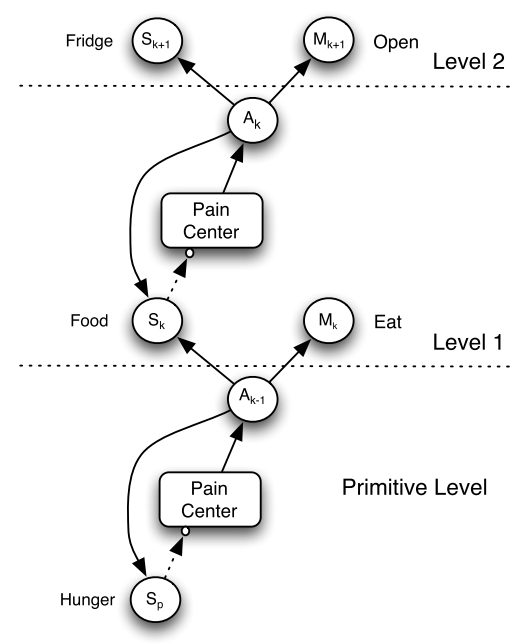
\includegraphics[width=0.5\linewidth]{rozdzial2/images/abstract_pains_creation}
	\caption{Tworzenie sygnałów abstrakcyjnych bóli. Źródło: 
	\cite{ml_dev_auto_systems}}
	\label{fig:abstractpainscreation}
\end{figure}

Bóle tworzą hierarchię wszerz i wgłąb, tworząc struktury grafowe. 
W takich strukturach teoretycznie mogą pojawiać się zamknięte ścieżki, np. brak
jedzenia może sprawić, żeby kupić więcej jedzenia, a do tego potrzebne są 
pieniądze, które można zdobyć sprzedając jedzenie. Należy wziąć pod uwagę takie 
sytuacje w procesie tworzenia całej architektury i sposobu uczenia maszyny.

\section{Tworzenie celów w uczeniu motywowanym}

Jednym z podstawowych źródeł tworzenia nowych celów jest wcześniej wspomniany 
ból. Najbardziej prymitywnym bólem u ludzi jest uczucie dyskomfortu, gdy czują 
głód. W maszynach można to odnieść do poziomu naładowania baterii w robocie i 
coraz niższy poziom sprawia, że ból związany z brakiem energii zwiększa się. 
Agent uczenia motywowanego musi się nauczyć jak ten ból zmniejszać, tak jak 
człowiek uczy się zdobywać jedzenie oraz jeść. Mimo, że wszelkie abstrakcyjne 
bóle, które wykształcają się w dalszym rozwoju, to te prymitywne umożliwiają 
realizację kolejnych zadań czy celów.

Dokładny opis algorytmu tworzenia celów został opisany w 
\cite{ml_comp_int}

\textbf{Algorytm tworzenia celów (ang. \textit{goal creation system})}
\begin{enumerate}
    \item Wybierz dominujący ból stosując regułę zwycięzca bierze wszystko 
        (ang. \textit{winner takes all}) spomiędzy konkurujących ośrodków bólu.
        \begin{itemize}
            \item Jeżeli żaden z bóli nie przekracza wcześniej zdefiniowanego 
                progu, czekaj aż któryś z nich przekroczy ten próg.
        \end{itemize}
    \item Jako aktualny cel wybierz zmniejszenie dominującego bólu.
        \begin{itemize}
            \item aktualny cel motywuje agenta do działania.
        \end{itemize}
    \item Wybierz wcześniej nauczoną akcje, która z najwyższym 
          prawdopodobieństwem spełni aktualny cel.
        \begin{itemize}
            \item Jeżeli nie ma żadnego, idź do punktu 6.
        \end{itemize}
    \item Sprawdź czy wybrana czynność może być wykonana w aktualnym środowisku. 
        Jeśli nie, idź do punktu 3.
    \item Wykonaj akcję.
        \begin{itemize}
            \item Jeśli ta akcja \textit{obniżyła} wartość dominującego bólu:
                \begin{enumerate}
                    \item Zwiększ wartości wag zależności pomiędzy aktualnym 
                        bólem a~akcją jaka została wykonana i~zwiększ wartość 
                        wag odpowiadających abstrakcyjnemu bólowi powiązanego 
                        z~tą akcją.
                    \item Idź do punktu 1.
                \end{enumerate}
            \item Jeśli ta akcja \textit{nie obniżyła} wartości dominującego bólu.
                \begin{enumerate}
                    \item Zmniejsz wartości wag zależności pomiędzy aktualnym 
                        bólem a~akcją jaka została wykonana i~zmniejsz wartość 
                        wag odpowiadających abstrakcyjnemu bólowi powiązanego 
                        z~tą akcją.
                    \item Idź do punktu 3.
                \end{enumerate}
        \end{itemize}
    \item Wykonaj eksplorację przestrzeni akcji mającą na celu spełnienie celu.
        \begin{itemize}
            \item Jeśli nowa akcja \textit{zmniejszyła} wartość dominującego bólu.
                \begin{enumerate}
                    \item Zwiększ wartości wag zależności pomiędzy aktualnym 
                        bólem a~akcją jaka została wykonana i~stwórz nowy 
                        abstrakcyjny ból związany z~niemożliwością wykonania 
                        tej akcji.
                    \item Idź do punktu 1.
                \end{enumerate}
            \item Jeśli nowa akcja \textit{nie zmniejszyła} wartości 
                dominującego bólu, idź do punktu 6.
        \end{itemize}
\end{enumerate}

Uczenie motywowane może być zastosowane wspólnie z~uczeniem opartym na 
ciekawości (ang. \textit{curiosity based learning}) -- ciekawość poinformuje 
agenta o~nowych odkryciach, podczas gdy uczenie motywowane skupi się na 
poszukiwaniu konkretnych celów, które nie są podane przez twórcę (tak jak 
w~uczeniu ze wzmocnieniem).

\section{Podstawowy element systemu tworzenia celów}

Mechanizm budowania celów składa się z wielu, prostych elementów nazywanych 
jednostkami tworzenia celów (ang. \textit{goal creation unit}). Składa się on 
głównie z trzech typów neuronów, które wchodzą ze sobą w interakcję. Są to:

\begin{itemize}
	\item neurony odpowiadające za ból (ang. \textit{pain center neurons}),
	\item neurony wzmacniające lub zmniejszające odczucie bólu (ang. 
	\textit{reinforcement neuro-transmitter neurons}),
	\item neurony odpowiadające za motorykę (ang. \textit{neurons in sensory 
	and motor pathway}).
\end{itemize}

Schemat reprezentujący połączenia zawarto na rysunku 
\ref{fig:goalcreationsystemunit}.

\begin{figure}[H]
	\centering
	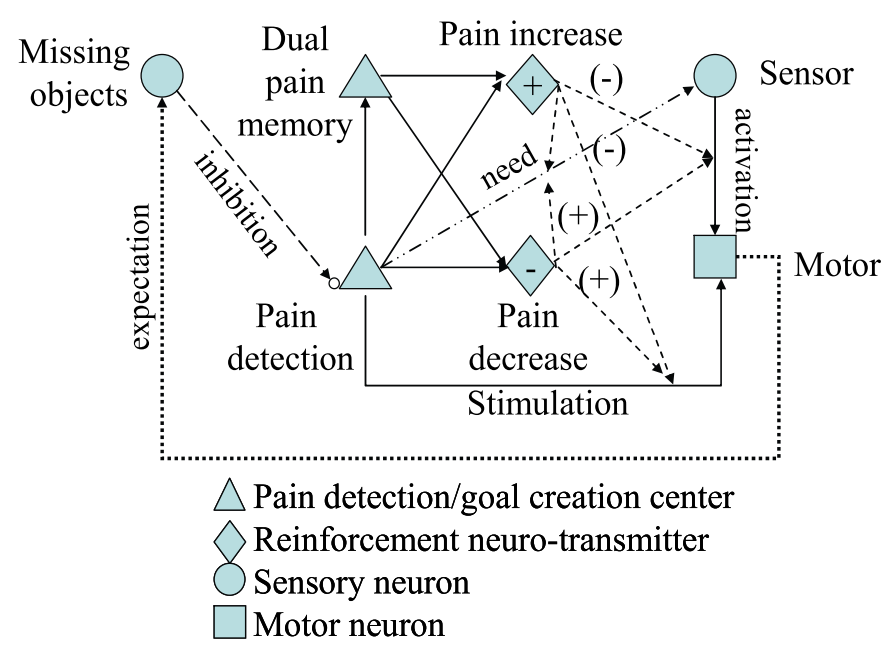
\includegraphics[width=0.7\linewidth]{rozdzial2/images/goal_creation_system_unit}
	\caption{Schemat podstawowego elementu systemu tworzenia celów. Źródło: 
	\cite{motivation_in_ei}.}
	\label{fig:goalcreationsystemunit}
\end{figure}

Neurony odpowiadające za odczuwanie bólu (te po lewej stronie na rysunku 
\ref{fig:goalcreationsystemunit}) są stymulowane przez sygnał reprezentujący 
ból oznaczany przez $I_P$. Reprezentuje on negatywny stymulant, np. ból, 
dyskomfort czy nieprzyjemność. Ponieważ ból istnieje z powodu braku czegoś w 
środowisku (oznaczone na rysunku jako "missing objects"), to neurony 
odpowiedzialne za detekcję bólu aktywują się w momencie wyciszenia neuronu 
odpowiedzialnego za czytanie wartości z otoczenia. Dodana została także pamięć 
wartości bólu z poprzedniego wydarzenia, oznaczone jako $I_{Pd}$. Neurony 
wykorzystują tą wartość do wzmacniania uczucia odczuwania bólu, jeżeli 
zwiększył się on od poprzedniego wydarzenia. Wartość tego wzmocnienia zapisano 
w równaniu \ref{equ:reinforcement_pain}.

\begin{equation}
	\label{equ:reinforcement_pain}
	r = I_P - I_{Pd}
\end{equation}

Ostatnią grupą (po prawej stronie na rysunku \ref{fig:goalcreationsystemunit}) 
są neurony odpowiedzialne za obliczanie wartości akcji jakie ma wykonać robot. 
Na początku centrum detekcji bólu bezpośrednio wpływa na neurony odpowiedzialne 
za wykonywanie akcji, ponieważ wszelkie wagi neuronów $W_{MP}$ są losowo 
zainicjalizowane. W trakcie poznawania środowiska, maszyna dostraja wartości 
tych wag. Dodatkowo, aby pewna akcja była wykonana muszą być dostępne pewne 
obiekty z otoczenia (na rysunku \ref{fig:goalcreationsystemunit} oznaczone jako 
"Sensor" po prawej stronie). Na początku neuron będzie miał powiązania z 
wieloma różnymi obiektami poprzez losowa zainicjalizowane wagi $W_{MS}$.

Po wykonanej akcji, która zmniejszyła albo zwiększyła wartość odczuwanego bólu 
(wykrytego przez drugą grupę neuronów odpowiedzialną za detekcję bólu), 
generowany jest sygnał $r$ (obliczony zgodnie z równaniem 
\ref{equ:reinforcement_pain}). Wykorzystywany jest to wzmocnienia lub 
osłabienia wag $W_{MP}$ i $W_{MS}$ zgodnie z równaniem \ref{equ:weights_update}

\begin{equation}
	\label{equ:weights_update}
	\begin{aligned}
		W_{MP} = W_{MP} + r \cdot \beta ^ n \\
		W_{MS} = W_{MS} + r \cdot \beta ^ n
	\end{aligned}
\end{equation}

gdzie:
\begin{itemize}
	\item $\beta$ -- oznacza współczynnik uczenia, mniejszy od wartości 1,
	\item $n$ -- oznacza jak wiele razy dane połączenie było zmieniane.
\end{itemize}

Dodatkowo neuron odpowiedzialny za reprezentację obiektu, który był użyty do 
zmniejszenia bólu zostanie dodany z wagą $W_{SP}$ w celu połączenia centrum 
detekcji bólu z neuronem sensorycznym. Ten neuron będzie uczony korzystając 
uczenia metodą Hebba.

Z kolei z drugiej strony, obiekt, którego zabrakło i stworzył on ból 
abstrakcyjny, staje się dostępny. Zostaje stworzony neuron reprezentujący 
połączenie neuronu odpowiedzialnego za motorykę z neuronem z brakującym 
obiektem z wagą $W_{SM}$.

Oba wymienione wcześniej połączone będą uczone metodą wzmocnienia. Oznacza to, 
że im mocniejsza zmiana poziomu bólu, tym mocniejsza korekta wartości tych wag. 




\chapter{Testy}

\section{Test URL-a}

Wejdź na stronę \url{https://www.google.pl/} i wpisz szukane zdanie.

\clearpage

\section{Test dzielenia wdów}

Lorem ipsum dolor sit amet, ex est alia dolorem commune. Duo modo errem no. Ea harum doming atomorum mei. Consul animal malorum cu qui, sumo dicta graece an est, vim ei clita regione.

Vel eu quando doming fastidii, mei graeco indoctum an, legere theophrastus in pro. Te mei probatus eleifend interpretaris. Est no autem liber vituperatoribus, cu mea dicam constituto. Ea laudem tritani consectetuer sit, sanctus patrioque expetendis vix in. Duo id fugit adversarium signiferumque, an quot modus molestiae qui.

Ut paulo definiebas pro. Mea an quod esse. Et atomorum facilisis moderatius sit. Graeco iudicabit forensibus in vel. Eam cu lorem aeterno offendit, cu vix nulla congue posidonium. Vel lucilius evertitur vituperata no.

Mea eu graecis prodesset. Et tota eius nec. Ei etiam oratio has, vel ei homero eripuit invenire. Sed ex errem intellegebat, sea et elitr intellegat constituto. Nostro voluptua accusamus eos in, ei sale admodum has. Vim ne consetetur reformidans, ad has malis recusabo persequeris, per etiam virtute invenire in.

Te nihil eruditi eam, sit aperiam accusam mediocritatem at. Nec ne nonumy dictas disputationi, vis ridens sadipscing ex. Harum euripidis ex vix, at consetetur instructior signiferumque mel, at mei elitr honestatis. Id sit congue vituperata. Temporibus eloquentiam no eum.

Pro id esse phaedrum, nostro iudicabit eos ut. Sit ea aperiam alienum, harum audiam voluptua cu usu. Iudico invenire te vel, id suscipit disputando pri. Ut sumo expetenda mea.

Cum at idque nullam aperiam, vis ex aeque ponderum luptatum. Vix soluta graeco dissentiet ut, ut est reque periculis similique, ut dicta dicant repudiare sea. Ne dolor legendos signiferumque ius, at eirmod convenire qui. Suas numquam conceptam mei ex. Autem homero eos et, sea dicta alienum iudicabit ut.

Ea duo consulatu vulputate, id elit perpetua cum. His ei aeque saepe audiam. Prompta laoreet facilisi ne sed, per hinc consetetur te, oratio fuisset ullamcorper mel at. Quis suscipiantur ne nec, agam efficiendi usu in.

Vis eu iuvaret singulis appellantur, usu ex saepe omittantur. Sed possit mnesarchum at, usu illum choro oratio in, et debet dolor vix. Mel aperiri suscipiantur ne, te per illum fuisset, lorem pericula mei ad. Pri id tale lucilius dissentiet, id sea sonet expetenda. Agam sensibus persequeris sed no, eum at tamquam sanctus.

Omnis exerci soleat ut vis. Rebum vidisse sea ex. Ius animal gubergren efficiantur ad, mollis probatus nec ut. Meis platonem ex vel, ut qui tale tritani equidem. Vide meis fuisset mel at, nam an assum delenit gubergren. No illum reprimique vim, te augue nullam per, ludus dicant suscipiantur ne sed.

An pri mediocrem deseruisse, ad sumo audire dissentiet sit. Sit ea civibus lobortis. Etiam ceteros commune ei vis. Pro ei equidem vivendo. Quo ne prima periculis omittantur, ex rebum veritus sit, ei dolor maiestatis mea.

\subsection{Lorem ipsum}

Et mel munere quodsi sapientem. Essent legimus ne pro. Est ornatus definiebas et. No habemus docendi ius, purto sapientem mei at. Tamquam vivendo necessitatibus has at, no habemus praesent nec. No quo modus iudicabit scriptorem. Modus intellegebat ea vim. Cu ius lorem regione offendit, ne accusata sensibus vituperatoribus quo. Sit ut iuvaret indoctum. Ut mea sale justo. Sapientem definitionem ius eu, at sea quem doming. Facete conclusionemque ut nec, vix at duis eius. Eos quot consequuntur et, ornatus liberavisse ne mei.

Per an dicam commodo tractatos, usu in timeam numquam tacimates. Case delectus eu sea, usu audiam eleifend tincidunt id, nec at decore discere mentitum. Ut elit veri eloquentiam his, ceteros tractatos ea has. Duo impetus scribentur et, eu quo errem everti, ad recusabo consulatu ius. Fastidii comprehensam pri ea, ex duo augue quando denique. Eos aeterno deserunt sententiae cu, ius quas tation patrioque ex.

Id autem scripta explicari nec, congue quidam possit te sit. Et usu ipsum bonorum graecis, ferri verear deterruisset eum cu. Purto porro accommodare cu vim. Cum ei tritani pertinacia voluptaria.



% itd.
% \appendix
% \include{dodatekA}
% \include{dodatekB}
% itd.

\printbibliography

\end{document}
